\documentclass[../main.tex]{subfiles}
\begin{document}
\begin{CJK*}{UTF8}{bkai}
\subsection{熱量輸送,非穩態問題}
\begin{itemize}
  \item 可分成兩種
  \begin{enumerate}
    \item 可忽略內部熱傳\\
      物體內部沒有溫度差,$T(r,t)\to T(t)$\\
      稱為Lump-capacitance model\\
      可忽略內部熱傳的原因:
      \begin{itemize}
        \item 物體體積很小
        \item 物體熱傳導係數很大
        \item 液體或氣體被均勻攪拌,故內部沒有溫度差
        \item Biot $\leq$ 0.1
      \end{itemize}
    \item 不可忽略內部熱傳\\
      內部有熱傳導,內部溫度不均一,$T(r,t)$\\
      使用Shell Balance或General Heat Transfer方法來求解
  \end{enumerate}
  \item Lump-capacitance model
  \begin{figure}[H]
    \centering
    \begin{tikzpicture}[>=Latex, line cap=round, line join=round, thick]
      \draw (0,0) circle (3);
      \draw [dashed, blue] (0,0) circle (2.9);
      \fill [pattern=dots, pattern color=blue] (0,0) circle (2.9);
      \draw[<->] (0,0) -- (225:3) node[below left] {$R$};
      \node[anchor=south, blue] at (0,3) {$C.V.$};
      \node[anchor=south] at (0,0) {$T(t)$};
      \node at (0,1) {$T(0)=T_0$};
      \draw[->, decorate, decoration=snake] (30:3) -- (30:4.5) node[midway, above=4pt] {$h$};
      \draw [dashed] (0,0) circle (4.5);
      \node[anchor=south west] at (4.5,0) {$T_{\infty}$};
      \draw[->, dashed] (0,0) -- (3,0) node[midway, above=6pt] {$\cancel{q_k}$};
      \draw (1.5,0) -- +(-0.2,0.2);
      \draw (1.5,0) -- +(-0.2,-0.2);
      \draw (1.5,0) -- +(0.2,0.2);
      \draw (1.5,0) -- +(0.2,-0.2);
      \draw[->, red] (3,0) -- (4.5,0) node[midway, above] {$q_c$};
    \end{tikzpicture}
    \caption{Lump-capacitance model示意圖}
  \end{figure}
  \begin{itemize}
    \item 使用Shell-Balance求解,假設整個物體溫度均一為$T(t)$\\
      故控制體積可以為整個物體
    \item 能量守恆式:
      \begin{equation}
        \cancel{ \dot{Q}_\text{in} }- \cancel{\dot{Q}_\text{out}} \pm \dot{Q}_\text{gen} = \rho C_V \frac{dT}{dt}
      \end{equation}
    \item 由於向外界散熱,並因為固體,假設$C_V=C_P$,假設熱容為定值,故能量平衡為:
      \begin{equation}
        -hA(T-T_{\infty}) =\rho C_P V \frac{dT}{dt}
      \end{equation}
    \item 分離變數並積分:
    \begin{align}
      -hA(T-T_{\infty}) &=\rho C_P V \frac{dT}{dt} \nonumber\\
      \frac{dT}{T-T_{\infty}} &= -\frac{hA}{\rho C_P V} dt \nonumber\\
      \int_{T_0}^{T(t)} \frac{dT}{T-T_{\infty}} &= -\frac{hA}{\rho C_P V} \int_0^t dt \nonumber\\
      \ln\left(\frac{T(t)-T_{\infty}}{T_0 - T_{\infty}}\right) &= -\frac{hA}{\rho C_P V} t \nonumber\\
      \therefore \quad \frac{T(t)-T_{\infty}}{T_0 - T_{\infty}} &= \exp\left(-\frac{hA}{\rho C_P V} t\right) \label{eq:heat_transfer_unsteady_lump_capacitance_model}
    \end{align}
    \item 故物體散熱隨時間的關係式:
    \begin{equation}
      \boxed{
        T(t) = T_{\infty} + (T_0 - T_{\infty}) \exp\left(-\frac{hA}{\rho C_P V} t\right)
      }
    \end{equation}
    P.S.也可以用General Heat Transfer Equation求得:
    \begin{equation}
      \rho C_P\left(\frac{\partial T}{\partial t}+\cancel{\vec{\bm u}}\cdot\nabla T\right) = \cancel{k\nabla^2T} \pm \dot{q}
    \end{equation}
    但注意這邊$\dot{q}$因為是放熱,所以是負號\\
    而且使用此式時會強迫三維(畢竟有$\nabla$),故$\dot q$項為$-\frac{q_c}{V}$\\
    故:
    \begin{equation}
      \rho C_P \frac{\partial T}{\partial t} = -\frac{hA(T-T_{\infty})}{V}
    \end{equation}
    與前面使用Shell Balance的結果相同
    \item 此方程式可做三件事情:
    \begin{enumerate}
      \item 已知時間$t$,求溫度$T(t)$
      \item 已知溫度$T$,求時間$t$
      \item 已知溫度$T_1$與$T_2$,求所需時間差$t_2 - t_1$
    \end{enumerate}
    \item 另外,注意到(\ref{eq:heat_transfer_unsteady_lump_capacitance_model})的指數部分\\
    因為在$\ln$中是無單位的,所以$\frac{hA t}{\rho C_P V}$必須是無單位的\\
    我們可以從中定義兩個無因次群
    \begin{equation}
      \frac{hAt}{\rho V C_P} = \left(
        \frac{h\frac{V}{A}}{k}
      \right)\left(
        \frac{kt}{\rho C_P \left(\frac{V}{A}\right)^2}
      \right) = Bi \cdot Fo
    \end{equation}
    前面是Biot數,後面則是Fourier數
    \begin{equation}
      \boxed{\text{Fo} = \frac{kt}{\rho C_P \left(\frac{V}{A}\right)^2} = \frac{\alpha t}{\left(\frac{V}{A}\right)^2}}
    \end{equation}
    Forier的物理意義,如果將分子分母同乘$\Delta V/L$,則變成:
    \begin{equation}
      \text{Fo} = \frac{kA\Delta T/L}{\rho V C_P \Delta T/t} = \frac{\text{熱傳導}}{\text{熱儲存速率}\dot{H}}
    \end{equation}
    而若是固體,則$\dot H = \dot U$\\
    Fourier Number的應用:
    \begin{itemize}
      \item 若Fourier Number\fbox{很大},代表傳導速率遠大於熱儲存速率,故物體\fbox{溫度變化很快}\\
      物體是易散熱材料,如金屬
      \item 若Fourier Number\fbox{很小},代表傳導速率遠小於熱儲存速率,故物體\fbox{溫度變化很慢}\\
      物體是難散熱材料,如木頭、塑膠
    \end{itemize}
  \end{itemize}
  \item 內部熱傳導不可忽略
  \begin{itemize}
    \item 使用Shell Balance或General Heat Transfer Equation求解
    \begin{itemize}
      \item Shell Balance\\
        對控制體積作能量平衡,並列出PDE方程式
      \item General Heat Transfer Equation\\
        直接使用GHTE列出PDE方程式
    \end{itemize}
    使用時機:
    \begin{itemize}
      \item 體積很大,$T(r,t)$
      \item $k$值很小
      \item 沒有均勻攪拌
      \item $\text{Bi}>0.1$,不可忽略內部熱傳
    \end{itemize}
    \begin{figure}[H]
      \centering
      \begin{tikzpicture}[>=Latex, line cap=round, line join=round, thick]
        \draw (0,0) rectangle (6,2);
        \fill[pattern=north east lines] (0,0) rectangle (6,-0.3);
        \fill[pattern=north east lines] (0,2.3) rectangle (6,2);
        \node[anchor=north] at (3,-0.3) {Insulated};
        \node[anchor=south] at (3,2.3) {Insulated};
        \draw[<->] (0,0.2) -- (6,0.2) node[midway, above] {$L$};
        \node at (3,3.2) {$T(x,t), T(x,0)=T_0>T_s$};
        \node[anchor=south] at (0,2.3) {$T_s$};
        \node[anchor=south] at (6,2.3) {$T_s$};
        \draw[dashed] (3,0.5) -- (3,1.5);
        \draw[->, decorate, decoration=snake] (3,1) -- (6,1) node[midway, above=4pt] {$q_k$};
        \draw[->, decorate, decoration=snake] (3,1) -- (0,1) node[midway, above=4pt] {$q_k$};
        \fill[pattern=crosshatch dots, pattern color=blue] (3.75,0) rectangle (4.25,2);
        \draw[blue, dashed] (3.75,0) -- (3.75,2);
        \draw[blue, dashed] (4.25,0) -- (4.25,2);
        \node[anchor=south west, blue] at (4.25,0.3) {C.V.};
        \draw (0,0) -- (0,-0.7);
        \draw [->] (0,-0.5) -- (1,-0.5) node[right] {$x$};
      \end{tikzpicture}
      \caption{不可忽略內部熱傳示意圖,末端溫度已知}
    \end{figure}
    \item 使用Shell Balance求解
    \begin{equation}
      \begin{matrix}
        Q_\text{in} & - & Q_\text{out}        & \pm & Q_\text{gen} & = & \text{Accumulation} \\
        q_k|_x A    &   & q_k|_{x+\Delta x} A &     & 0 &&\\
        0           & & 0 && 0 &&
      \end{matrix}
    \end{equation}
    注意因為是絕緣,所以對流會被放在邊界條件,而不是控制體積內
    \begin{align}
      q_k|_x A - q_k|_{x+\Delta x} A &= \rho C_P A \Delta x \frac{\partial T}{\partial t} \nonumber\\
      -\frac{\partial q_k}{\partial x} \Delta x A &= \rho C_P A \Delta x \frac{\partial T}{\partial t} \nonumber\\
      -\frac{\partial}{\partial x}\left(-k \frac{\partial T}{\partial x}\right) &= \rho C_P \frac{\partial T}{\partial t} \nonumber\\
      k \frac{\partial^2 T}{\partial x^2} &= \rho C_P \frac{\partial T}{\partial t} \nonumber\\
      \therefore \quad \frac{\partial T}{\partial t} &= \alpha \frac{\partial^2 T}{\partial x^2} \label{eq:heat_transfer_unsteady_internal_conduction_PDE}
    \end{align}
    此為傅立葉第二定律\\
    而邊界條件為:
    \begin{align}
      T(x,0) &= T_0 \label{eq:heat_transfer_unsteady_internal_conduction_BC1}\\
      T(0,t) &= T_s \label{eq:heat_transfer_unsteady_internal_conduction_BC2}\\
      T(L,t) &= T_s \label{eq:heat_transfer_unsteady_internal_conduction_BC3}
    \end{align}
    P.S. 此外上式也可以用General Heat Transfer Equation求解:
    \begin{equation}
      \rho C_P \left(
        \frac{\partial T}{\partial t} + \cancel{\vec{\bm u}}\cdot\nabla T
      \right) = k \nabla^2 T \pm \cancel{\dot{q}}
    \end{equation}
    因為沒有對流與熱源,所以被消掉\\
    得到:
    \begin{equation}
      \rho C_P \frac{\partial T}{\partial t} = k \frac{\partial^2 T}{\partial x^2}
    \end{equation}
    與前面使用Shell Balance的結果相同
    \item 求解,為標準S-L問題
    \begin{enumerate}
      \item 分離變數:
      \begin{equation}
        T(x,t) = X(x) \tau(t)
      \end{equation}
      \item 帶入PDE(\ref{eq:heat_transfer_unsteady_internal_conduction_PDE}):
      \begin{equation}
        X \frac{d\tau}{dt} = \alpha \tau \frac{d^2 X}{dx^2}
      \end{equation}
      \item 分離變數,並令等號為$-\lambda^2$:
      \begin{equation}
        \frac{1}{\alpha \tau} \frac{d\tau}{dt} = \frac{1}{X} \frac{d^2 X}{dx^2} = -\lambda^2
      \end{equation}
      \item 得到兩個ODE:
      \begin{align}
        \frac{d\tau}{dt} + \alpha \lambda^2 \tau &= 0 \label{eq:heat_transfer_unsteady_internal_conduction_ODE1}\\
        \frac{d^2 X}{dx^2} + \lambda^2 X &= 0 \label{eq:heat_transfer_unsteady_internal_conduction_ODE2}
      \end{align}
      \item 因為會有特殊解,要用邊界條件來規範各特徵解的係數,所以從時間開始解起
      \begin{equation}
        \tau(t) = C e^{-\alpha \lambda^2 t}
      \end{equation}
      \item 空間ODE(\ref{eq:heat_transfer_unsteady_internal_conduction_ODE2})的通解:
      \begin{equation}
        X(x) = A \cos (\lambda x) + B \sin (\lambda x)
      \end{equation}
      \item 代入邊界條件(\ref{eq:heat_transfer_unsteady_internal_conduction_BC2})(\ref{eq:heat_transfer_unsteady_internal_conduction_BC3}):
      \begin{align}
        X(0) &= T_s \Rightarrow A = T_s \\
        X(L) &= T_s \Rightarrow B \sin( \lambda L) = 0
      \end{align}
      \item 故特徵值為:
      \begin{equation}
        \lambda_n = \frac{n\pi}{L} \quad n=1,2,3,...
      \end{equation}
      \item 故所有特徵解為:
      \begin{equation}
        T_n(x,t) = \left[
          T_s + B_n \sin\left(\frac{n\pi}{L} x\right)
        \right] e^{-\alpha \left(\frac{n\pi}{L}\right)^2 t}
      \end{equation}
      \item 最後利用正交性,並用初始條件(\ref{eq:heat_transfer_unsteady_internal_conduction_BC1})求出各係數$B_n$:
      \begin{align}
        T(x,0) = T_0 &= T_s + \sum_{n=1}^\infty B_n \sin\left(\frac{n\pi}{L} x\right) \nonumber\\
        T_0 - T_s &=\sum_{n=1}^\infty B_n \sin\left(\frac{n\pi}{L} x\right)
      \end{align}
      代入正交的積分:
      \begin{align}
        \int_0^L (T_0 - T_s) \sin\left(\frac{m\pi}{L} x\right) dx &= 
        \sum_{n=1}^\infty B_n \int_0^L \sin\left(\frac{n\pi}{L} x\right) \sin\left(\frac{m\pi}{L} x\right) dx \nonumber\\
        &= B_m \frac{L}{2} \nonumber\\
        \therefore \quad B_m &= \frac{2}{L} \int_0^L (T_0 - T_s) \sin\left(\frac{m\pi}{L} x\right) dx
      \end{align}
      \item 計算積分:
      \begin{align}
        B_n &= \frac{2}{L} \int_0^L (T_0 - T_s) \sin\left(\frac{n\pi}{L} x\right) dx \nonumber\\
        &= \frac{2(T_0 - T_s)}{n\pi} \left[
          1 - \cos(n\pi)
        \right] \nonumber\\
        &= \begin{cases}
          \frac{4(T_0 - T_s)}{n\pi} & n\text{為奇數}\\
          0 & n\text{為偶數}
        \end{cases}
      \end{align}
      \item 故最後解為:
      \begin{equation}
        \boxed{
          T(x,t) = T_s + \sum_{m=2n+1}^{\infty} \frac{4(T_0 - T_s)}{m\pi} 
          \sin\left(\frac{m\pi}{L} x\right) e^{-\alpha \left(\frac{m\pi}{L}\right)^2 t}
        }
      \end{equation}
    \end{enumerate}
    \item 如果邊界條件改成不知道末端的溫度
    \begin{figure}[H]
      \centering
      \begin{tikzpicture}[>=Latex, line cap=round, line join=round, thick]
        \draw (0,0) rectangle (6,2);
        \node at (-1,1) {$T_\infty$};
        \fill[pattern=north east lines] (0,0) rectangle (6,-0.3);
        \fill[pattern=north east lines] (0,2.3) rectangle (6,2);
        \node[anchor=north] at (3,-0.3) {Insulated};
        \node[anchor=south] at (3,2.3) {Insulated};
        \draw[<->] (0,0.2) -- (6,0.2) node[midway, above] {$L$};
        \node at (3,3.2) {$T(x,t), T(x,0)=T_0>T_\infty$};
        \node at (7,1) {$T_\infty$};
        \draw[dashed] (-0.5, 0) -- (-0.5,2);
        \draw[dashed] (6.5, 0) -- (6.5,2);
        \draw[dashed] (3,0.5) -- (3,1.5);
        \draw[->, decorate, decoration=snake] (3,1) -- (6,1) node[midway, above=4pt] {$q_k$};
        \draw[->, decorate, decoration=snake] (3,1) -- (0,1) node[midway, above=4pt] {$q_k$};
        \fill[pattern=crosshatch dots, pattern color=blue] (3.75,0) rectangle (4.25,2);
        \draw[blue, dashed] (3.75,0) -- (3.75,2);
        \draw[blue, dashed] (4.25,0) -- (4.25,2);
        \node[anchor=south west, blue] at (4.25,0.3) {C.V.};
        \draw (0,0) -- (0,-0.7);
        \draw [->] (0,-0.5) -- (1,-0.5) node[right] {$x$};
      \end{tikzpicture}
      \caption{不可忽略內部熱傳示意圖,末端對流邊界條件}
    \end{figure}
    \item 邊界條件變成:
    \begin{align}
      T(x,0) &= T_0 \label{eq:heat_transfer_unsteady_internal_conduction_BC4}\\
      -k \left.\frac{\partial T}{\partial x}\right|_{x=0} &= h \left[
        T(0,t) - T_{\infty}
      \right] \label{eq:heat_transfer_unsteady_internal_conduction_BC5}\\
      k \left.\frac{\partial T}{\partial x}\right|_{x=L} &= h \left[
        T(L,t) - T_{\infty}
      \right] \label{eq:heat_transfer_unsteady_internal_conduction_BC6}
    \end{align}
    \item 由於這種對稱性又扯到微分的題目很麻煩,所以重新定義$L$和原點使其對稱\\
    令總長為$2L$,原點在中間\\
    邊界條件改為(因為對稱性,所以第三個會變成刪除奇函數用)\\
    然後多出一條中間必須要連續的條件:
    \begin{align}
      T(x,0) &= T_0 \label{eq:heat_transfer_unsteady_internal_conduction_BC7}\\
      -k \left.\frac{\partial T}{\partial x}\right|_{x=-L} &= h \left[
        T(-L,t) - T_{\infty}
      \right] \label{eq:heat_transfer_unsteady_internal_conduction_BC8}\\
      -k \left.\frac{\partial T}{\partial x}\right|_{x=L} &= h \left[
        T(L,t) - T_{\infty}
      \right] \label{eq:heat_transfer_unsteady_internal_conduction_BC9}\\
      \left.\frac{\partial T}{\partial x}\right|_{x=0} &= 0 \label{eq:heat_transfer_unsteady_internal_conduction_BC10}
    \end{align}
    \item 求解S-L問題
    \begin{enumerate}
      \item 分離變數:
      \begin{equation}
        T(x,t) = X(x) \tau(t)
      \end{equation}
      \item 帶入PDE(\ref{eq:heat_transfer_unsteady_internal_conduction_PDE}):
      \begin{equation}
        X \frac{d\tau}{dt} = \alpha \tau \frac{d^2 X}{dx^2}
      \end{equation}
      \item 分離變數,並令等號為$-\lambda^2$:
      \begin{equation}
        \frac{1}{\alpha \tau} \frac{d\tau}{dt} = \frac{1}{X} \frac{d^2 X}{dx^2} = -\lambda^2
      \end{equation}
      \item 得到兩個ODE:
      \begin{align}
        \frac{d\tau}{dt} + \alpha \lambda^2 \tau &= 0 \label{eq:heat_transfer_unsteady_internal_conduction_ODE3}\\
        \frac{d^2 X}{dx^2} + \lambda^2 X &= 0 \label{eq:heat_transfer_unsteady_internal_conduction_ODE4}
      \end{align}
      \item 先解時間ODE:
      \begin{equation}
        \tau(t) = C e^{-\alpha \lambda^2 t}
      \end{equation}
      \item 空間ODE(\ref{eq:heat_transfer_unsteady_internal_conduction_ODE4})的通解:
      \begin{equation}  
        X(x) = A \cos (\lambda x) + B \sin (\lambda x)
      \end{equation}
      \item 故通解為:
      \begin{equation}
        T(x,t) = \left[
          A \cos (\lambda x )+ B \sin (\lambda x)
        \right] e^{-\alpha \lambda^2 t}
      \end{equation}
      由於對稱性,為偶函數,故$B=0$\\
      等同於用去(\ref{eq:heat_transfer_unsteady_internal_conduction_BC10}和\ref{eq:heat_transfer_unsteady_internal_conduction_BC10})消去奇函數
      \item 代入邊界條件(\ref{eq:heat_transfer_unsteady_internal_conduction_BC9})
      \begin{equation}
        -k \left.\frac{\partial T}{\partial x}\right|_{x=L} = h \left[
          T(L,t) - T_{\infty}
        \right]
      \end{equation}
      \item 變數代換,令$\theta = T-T_\infty$
      \begin{equation}
       - k \left.\frac{\partial \theta}{\partial x}\right|_{x=L} = h \left[
          \theta(L,t)
        \right]
      \end{equation}
      而
      \begin{align}
        \theta(x,t) &= T(x,t) - T_\infty \nonumber\\
        &= \left[
          A \cos (\lambda x)
        \right] e^{-\alpha \lambda^2 t} - T_\infty \nonumber\\
        \therefore \quad \frac{\partial \theta}{\partial x} &= -A \lambda \sin (\lambda x) e^{-\alpha \lambda^2 t}
      \end{align}
      代回去:
      \begin{align}
        -k \left(
          -A \lambda \sin (\lambda L) e^{-\alpha \lambda^2 t}
        \right) &= h \left(
          A \cos (\lambda L) e^{-\alpha \lambda^2 t}
        \right) \nonumber\\
        k A \lambda \sin (\lambda L) &= h A \cos (\lambda L )\nonumber\\
        k \lambda \sin (\lambda L) &= h \cos (\lambda L) \nonumber\\
        \cot (\lambda L) &= \frac{k \lambda}{h}
      \end{align}
      同Bessel,又是一個在圖上找交點的問題
      \begin{figure}[H]
        \centering
        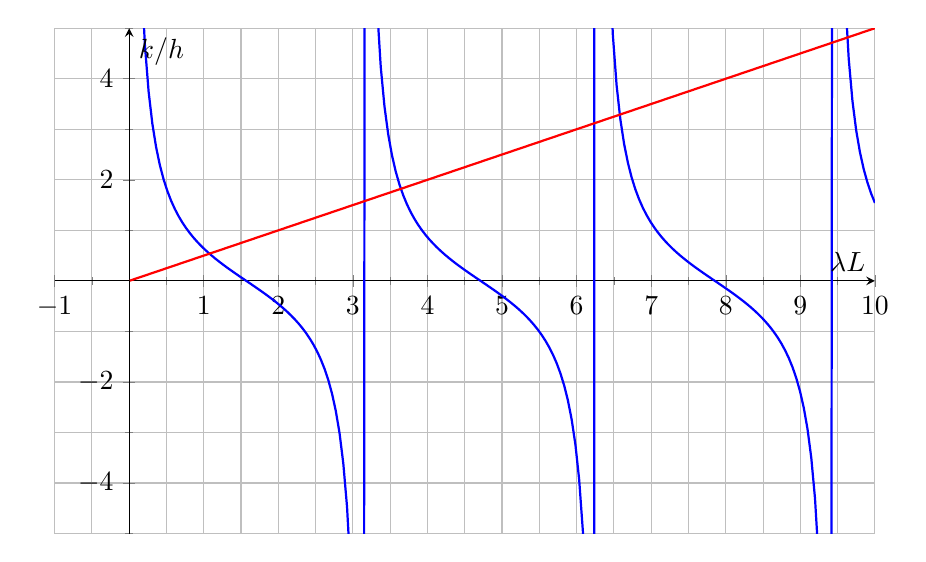
\begin{tikzpicture}
          \begin{axis}[
            axis lines = middle,
            xlabel = {$\lambda L$},
            ylabel = {$k/h$},
            ymin = -5, ymax = 5,
            xmin = -1, xmax = 10,
            domain=0.01:10,
            samples=200,
            width=12cm,
            height=8cm,
            grid=both,
            minor tick num=1,
            ]
            \addplot[blue, thick] {cot(deg(x))};
            \addplot[red, thick] {x/2}; 
          \end{axis}
        \end{tikzpicture}
        \caption{非穩態、熱傳,cot特徵值的圖解法示意圖}
      \end{figure}
      \item 但不管如何,我們知道了每個$\lambda_n$,只是沒有代數的描述而已
      \item 將所有特徵值代入,得到所有特徵解:
      \begin{equation}
        \theta_n(x,t) = A_n \cos (\lambda_n x) \cdot e^{-\alpha \lambda_n^2 t}
      \end{equation}
      \item 最後利用正交性,並用初始條件(\ref{eq:heat_transfer_unsteady_internal_conduction_BC7})求出各係數$A_n$:
      \begin{align}
        \theta(x,0) = T_0 - T_\infty = \sum_{n=1}^\infty A_n \cos (\lambda_n x) 
      \end{align}
      代入正交的積分:
      \begin{align}
        \int_{-L}^{L} (T_0 - T_\infty) \cos (\lambda_m x) dx &= 
        \sum_{n=1}^\infty A_n \int_{-L}^{L} \cos (\lambda_n x) \cos (\lambda_m x)  dx \nonumber\\
        &= A_m L \left(
          1 + \frac{\sin (2 \lambda_m L)}{2 \lambda_m L}
        \right) \nonumber\\
        \therefore \quad A_m &= \frac{1}{L \left(
          1 + \frac{\sin( 2 \lambda_m L)}{2 \lambda_m L}
        \right)} \int_{-L}^{L} (T_0 - T_\infty) \cos (\lambda_m x)  dx
      \end{align}
      \item 計算積分:
      \begin{align}
        A_n &= \frac{1}{L \left(
          1 + \frac{\sin 2 (\lambda_n L)}{2 \lambda_n L}
        \right)} \int_{-L}^{L} (T_0 - T_\infty) \cos (\lambda_n x) dx \nonumber\\
        &= \frac{2(T_0 - T_\infty)}{L \left(
          1 + \frac{\sin 2( \lambda_n L)}{2 \lambda_n L}
        \right)} \cdot \frac{\sin (\lambda_n L)}{\lambda_n} \nonumber\\
        &= \frac{2(T_0 - T_\infty) \sin (\lambda_n L)}{\lambda_n L \left(
          1 + \frac{\sin( 2 \lambda_n L)}{2 \lambda_n L}
        \right)}
      \end{align}
      \item 故最後解為:
      \begin{equation}
        \boxed{
          T(x,t) = T_\infty + \sum_{n=1}^\infty 
          \frac{2(T_0 - T_\infty) \sin( \lambda_n L)}{\lambda_n L \left(
            1 + \frac{\sin 2 \lambda_n L}{2 \lambda_n L}
          \right)} \cos (\lambda_n x) \cdot e^{-\alpha \lambda_n^2 t}
        }
      \end{equation}
    \end{enumerate}
    \item 假設長度無限長的熱傳\\
    Semi-infinite solid heat conduction
    \begin{figure}[H]
      \centering
      \begin{tikzpicture}[>=Latex, line cap=round, line join=round, thick]
        \draw (0,0) rectangle (8,2);
        \fill[pattern=north east lines, pattern color=red] (0,0) rectangle (-0.3,2);
        \draw[red, dashed] (0,0) -- (-0.3,0) -- (-0.3,2) -- (0,2);
        \fill[pattern=north east lines] (0,0) rectangle (8,-0.3);
        \fill[pattern=north east lines] (0,2.3) rectangle (8,2);
        \fill[white] (5.5,-0.5) .. controls (6,1) and (5,1) .. (5.5,2.5)
         -- (5.9,2.5) .. controls (5.4,1) and (6.4,1) .. (5.9,-0.5) -- cycle;
        \draw[dashed] (5.5,-0.5) .. controls (6,1) and (5,1) .. (5.5,2.5);
        \draw[dashed] (5.9,2.5) .. controls (5.4,1) and (6.4,1) .. (5.9,-0.5);
        \node at (4,3.2) {$T(x,t), T(x,0)=T_\infty$};
        \node[anchor=east, red] at (-0.3,1) {$T_0$};
        \draw[decorate, decoration=snake] (0,1) -- (7.5,1);
        \draw[->] (7.5,1) -- (8,1) node[right] {$x=\infty$};
        \fill[pattern=crosshatch dots, pattern color=blue] (3.75,0) rectangle (4.25,2);
        \draw[blue, dashed] (3.75,0) -- (3.75,2);
        \draw[blue, dashed] (4.25,0) -- (4.25,2);
        \node[anchor=south west, blue] at (4.25,0.3) {C.V.};
        \draw (0,0) -- (0,-0.7);
        \draw [->] (0,-0.5) -- (1,-0.5) node[right] {$x$};
      \end{tikzpicture}
      \caption{Semi-infinite solid heat conduction示意圖}
    \end{figure}
    一開始一個已經熱平衡為$T_\infty$的無限長固體\\
    在$t=0$時,將$x=0$處的溫度突然改為$T_0>T_\infty$\\
    求固體內部隨時間的溫度變化
    \item 邊界條件:
    \begin{align}
      T(x,0) &= T_\infty \label{eq:heat_transfer_unsteady_semi_infinite_BC1}\\
      T(0,t) &= T_0 \label{eq:heat_transfer_unsteady_semi_infinite_BC2}\\
      T(\infty,t) &= T_\infty \label{eq:heat_transfer_unsteady_semi_infinite_BC3}
    \end{align}
    這種有三個非齊次的,想辦法找到一個$\theta$,讓全部可以變成齊次或1\\
    令
    \begin{equation}
      \theta(x,t) = \frac{T(x,t) - T_\infty}{T_0 - T_\infty}
    \end{equation}
    則邊界條件變成:
    \begin{align}
      \theta(x,0) &= 0 \label{eq:heat_transfer_unsteady_semi_infinite_BC4}\\
      \theta(0,t) &= 1 \label{eq:heat_transfer_unsteady_semi_infinite_BC5}\\
      \theta(\infty,t) &= 0 \label{eq:heat_transfer_unsteady_semi_infinite_BC6}
    \end{align}
    \item 同上,Governal Heat Transfer Equation:
    \begin{equation}
      \frac{\partial T}{\partial t} = \alpha \frac{\partial^2 T}{\partial x^2}
    \end{equation}
    代入$\theta$:
    \begin{equation}
      \frac{\partial \theta}{\partial t} = \alpha \frac{\partial^2 \theta}{\partial x^2}
    \end{equation}
    這裡會使用Similarity Solution來解\\
    因為\fbox{分離變數後的邊界條件要都是齊次},所以無法使用分離變數法
    \item 令無因次變數:(原理同(\ref{sec:fluid_unsteady}))
    \begin{equation}
      \eta = \frac{x}{\sqrt{4 \alpha t}}
    \end{equation}
    \item 則:
    \begin{align}
      \frac{\partial \theta}{\partial t} &= \frac{d\theta}{d\eta} \cdot \frac{\partial \eta}{\partial t} = \frac{d\theta}{d\eta} \cdot \left(
        -\frac{x}{2 \sqrt{4 \alpha t^3}}
      \right) = -\frac{\eta}{2t} \frac{d\theta}{d\eta} \nonumber\\
      \frac{\partial \theta}{\partial x} &= \frac{d\theta}{d\eta} \cdot \frac{\partial \eta}{\partial x} = \frac{d\theta}{d\eta} \cdot \left(
        \frac{1}{\sqrt{4 \alpha t}}
      \right) = \frac{1}{\sqrt{4 \alpha t}} \frac{d\theta}{d\eta} \nonumber\\
      \frac{\partial^2 \theta}{\partial x^2} &= \frac{\partial}{\partial x} \left(
        \frac{1}{\sqrt{4 \alpha t}} \frac{d\theta}{d\eta}
      \right) = \frac{1}{4 \alpha t} \frac{d^2 \theta}{d\eta^2}
    \end{align}
    \item 代入PDE:
    \begin{align}
      -\frac{\eta}{2t} \frac{d\theta}{d\eta} &= \alpha \cdot \frac{1}{4 \alpha t} \frac{d^2 \theta}{d\eta^2} \nonumber\\
      - 2 \eta \frac{d\theta}{d\eta} &= \frac{d^2 \theta}{d\eta^2}
    \end{align}
    \item 這是一個ODE,可以用變數代換法解
    \begin{equation}
      \frac{d^2 \theta}{d\eta^2} + 2 \eta \frac{d\theta}{d\eta} = 0
    \end{equation}
    令
    \begin{equation}
      \frac{d\theta}{d\eta} = y
    \end{equation}
    則
    \begin{equation}
      \frac{d^2 \theta}{d\eta^2} = \frac{dy}{d\eta}
    \end{equation}
    \item 帶入ODE:
    \begin{equation}
      \frac{dy}{d\eta} + 2 \eta y = 0
    \end{equation}
    \item 使用積分因子法解ODE
    \begin{equation}
      \mu(\eta) = e^{\int 2 \eta d\eta} = e^{\eta^2}
    \end{equation}
    \item 代入:
    \begin{align}
      e^{\eta^2} \frac{dy}{d\eta} + 2 \eta e^{\eta^2} y &= 0 \nonumber\\
      \frac{d}{d\eta} \left(
        y e^{\eta^2}
      \right) &= 0 \nonumber\\
      y e^{\eta^2} &= C_1 \nonumber\\
      \therefore \quad y &= C_1 e^{-\eta^2}
    \end{align}
    \item 回代$y = \frac{d\theta}{d\eta}$:
    \begin{align}
      \frac{d\theta}{d\eta} &= C_1 e^{-\eta^2} \nonumber\\
      \theta &= C_1 \int e^{-\eta^2} d\eta + C_2
    \end{align}
    \item 使用誤差函數定義:
    \begin{equation}
      \operatorname{erf}(z) = \frac{2}{\sqrt{\pi}} \int_0^z e^{-s^2} ds
    \end{equation}
    \item 則:
    \begin{equation}
      \theta(\eta) = C_1 \cdot \frac{\sqrt{\pi}}{2} \text{erf}(\eta) + C_2
    \end{equation}
    \item 代入邊界條件(\ref{eq:heat_transfer_unsteady_semi_infinite_BC4})
    (\ref{eq:heat_transfer_unsteady_semi_infinite_BC5})(\ref{eq:heat_transfer_unsteady_semi_infinite_BC6}):\\
    $\theta(x,0)=0 \Rightarrow \theta(\eta \to \infty) = 0$
    \begin{align}
      0 &= C_1 \cdot \frac{\sqrt{\pi}}{2} \text{erf}(\infty) + C_2 \nonumber\\
      &= C_1 \cdot \frac{\sqrt{\pi}}{2} \cdot 1 + C_2 \nonumber\\
      \therefore \quad C_2 &= - C_1 \cdot \frac{\sqrt{\pi}}{2}
    \end{align}
    $\theta(0,t) = 1 \Rightarrow \theta(\eta=0) = 1$
    \begin{align}
      1 &= C_1 \cdot \frac{\sqrt{\pi}}{2} \text{erf}(0) + C_2 \nonumber\\
      &= 0 + C_2 \nonumber\\
      \therefore \quad C_2 &= 1
    \end{align}
    故:
    \begin{equation}
      - C_1 \cdot \frac{\sqrt{\pi}}{2} = 1 \Rightarrow C_1 = -\frac{2}{\sqrt{\pi}}
    \end{equation}
    \item 最後解為:
    \begin{equation}
      \theta(\eta) = 1 - \text{erf}(\eta) = \text{erfc}(\eta)
    \end{equation}
    \item 回代$\theta$:
    \begin{equation}
      \boxed{
        T(x,t) = T_\infty + (T_0 - T_\infty) \text{erfc} \left(
          \frac{x}{\sqrt{4 \alpha t}}
        \right)
      }
    \end{equation}
  \end{itemize}
\end{itemize}
\end{CJK*}
\end{document}